% Sketch output, version 0.2 (build 9, Thu Feb 8 22:06:23 2007)
% Output language: PGF/TikZ
\documentclass[letterpaper,12pt]{article}
\usepackage[x11names,rgb]{xcolor}
\usepackage{tikz}
\usetikzlibrary{snakes}
\usetikzlibrary{arrows}
\usetikzlibrary{shapes}
\usetikzlibrary{backgrounds}
\usepackage{amsmath}
\oddsidemargin 0in
\evensidemargin 0in
\topmargin 0in
\headheight 0in
\headsep 0in
\textheight 9in
\textwidth 6.5in
\begin{document}
\pagestyle{empty}
\vspace*{\fill}
\begin{center}
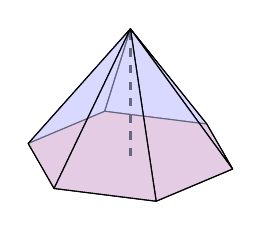
\begin{tikzpicture}[join=round]
\filldraw[fill=blue!20,fill opacity=0.5](0,1.619)--(-1.298,.162)--(-.327,.571)--(0,1.619)--cycle;
\filldraw[fill=blue!20,fill opacity=0.5](0,1.619)--(-.327,.571)--(.97,.409)--(0,1.619)--cycle;
\filldraw[fill=red!20](1.298,-.162)--(.97,.409)--(-.327,.571)--(-1.298,.162)--(-.97,-.409)--(.327,-.571)--cycle;
\filldraw[fill=blue!20,fill opacity=0.5](0,1.619)--(.97,.409)--(1.298,-.162)--(0,1.619)--cycle;
\filldraw[fill=blue!20,fill opacity=0.5](0,1.619)--(-.97,-.409)--(-1.298,.162)--(0,1.619)--cycle;
\draw[draw=black,dashed,line width=.8pt](0,0)--(0,1.619);
\filldraw[fill=blue!20,fill opacity=0.5](0,1.619)--(1.298,-.162)--(.327,-.571)--(0,1.619)--cycle;
\filldraw[fill=blue!20,fill opacity=0.5](0,1.619)--(.327,-.571)--(-.97,-.409)--(0,1.619)--cycle;
\end{tikzpicture}
\end{center}
\vspace*{\fill}
\end{document}
% End sketch output
